\documentclass[]{article}
\usepackage{lmodern}
\usepackage{amssymb,amsmath}
\usepackage{ifxetex,ifluatex}
\usepackage{fixltx2e} % provides \textsubscript
\ifnum 0\ifxetex 1\fi\ifluatex 1\fi=0 % if pdftex
  \usepackage[T1]{fontenc}
  \usepackage[utf8]{inputenc}
\else % if luatex or xelatex
  \ifxetex
    \usepackage{mathspec}
  \else
    \usepackage{fontspec}
  \fi
  \defaultfontfeatures{Ligatures=TeX,Scale=MatchLowercase}
\fi
% use upquote if available, for straight quotes in verbatim environments
\IfFileExists{upquote.sty}{\usepackage{upquote}}{}
% use microtype if available
\IfFileExists{microtype.sty}{%
\usepackage{microtype}
\UseMicrotypeSet[protrusion]{basicmath} % disable protrusion for tt fonts
}{}
\usepackage[margin=1in]{geometry}
\usepackage{hyperref}
\hypersetup{unicode=true,
            pdftitle={Higher number of bacterial colonies and morphotypes found in the cell phones of regular college students in comparison to nursing college students},
            pdfauthor={Angela Jocson},
            pdfborder={0 0 0},
            breaklinks=true}
\urlstyle{same}  % don't use monospace font for urls
\usepackage{longtable,booktabs}
\usepackage{graphicx,grffile}
\makeatletter
\def\maxwidth{\ifdim\Gin@nat@width>\linewidth\linewidth\else\Gin@nat@width\fi}
\def\maxheight{\ifdim\Gin@nat@height>\textheight\textheight\else\Gin@nat@height\fi}
\makeatother
% Scale images if necessary, so that they will not overflow the page
% margins by default, and it is still possible to overwrite the defaults
% using explicit options in \includegraphics[width, height, ...]{}
\setkeys{Gin}{width=\maxwidth,height=\maxheight,keepaspectratio}
\IfFileExists{parskip.sty}{%
\usepackage{parskip}
}{% else
\setlength{\parindent}{0pt}
\setlength{\parskip}{6pt plus 2pt minus 1pt}
}
\setlength{\emergencystretch}{3em}  % prevent overfull lines
\providecommand{\tightlist}{%
  \setlength{\itemsep}{0pt}\setlength{\parskip}{0pt}}
\setcounter{secnumdepth}{0}
% Redefines (sub)paragraphs to behave more like sections
\ifx\paragraph\undefined\else
\let\oldparagraph\paragraph
\renewcommand{\paragraph}[1]{\oldparagraph{#1}\mbox{}}
\fi
\ifx\subparagraph\undefined\else
\let\oldsubparagraph\subparagraph
\renewcommand{\subparagraph}[1]{\oldsubparagraph{#1}\mbox{}}
\fi

%%% Use protect on footnotes to avoid problems with footnotes in titles
\let\rmarkdownfootnote\footnote%
\def\footnote{\protect\rmarkdownfootnote}

%%% Change title format to be more compact
\usepackage{titling}

% Create subtitle command for use in maketitle
\providecommand{\subtitle}[1]{
  \posttitle{
    \begin{center}\large#1\end{center}
    }
}

\setlength{\droptitle}{-2em}

  \title{Higher number of bacterial colonies and morphotypes found in the cell
phones of regular college students in comparison to nursing college
students}
    \pretitle{\vspace{\droptitle}\centering\huge}
  \posttitle{\par}
    \author{Angela Jocson}
    \preauthor{\centering\large\emph}
  \postauthor{\par}
      \predate{\centering\large\emph}
  \postdate{\par}
    \date{Novemeber 16, 2019}


\begin{document}
\maketitle

\hypertarget{introduction}{%
\section{Introduction}\label{introduction}}

Cell phones have become an essential tool for modern-day life; in fact,
most people tend to not leave the house unless they have their cell
phone present. With cell phones becoming more a necessity rather than an
accessory, it is interesting to see how much bacteria our cell phones
can collect from our daily lives. In fact, in a 2014 study done by
Meadow et. al, they found that about 22\% of the bacterial taxa on
participants' fingers were also present on their own phones, as compared
to 17\% they shared on average with other people's phones (Meadow
\emph{et al.}, 2014). Meadow et. al's study implies that not only do
cell phones hold potential as carriers to our microbiome bacteria, but
also to all types of bacteria that are encountered throughout daily
life.

This idea is more worrisome when considering how much bacteria our cell
phones can bring in, especially when working in expectedly sterile
environments such as hospitals or emergency rooms. Karabay et. al (2007)
found that health professionals in a teaching hospital in Turkey carried
around cell phones that did get contaminated with bacteria, such as
\emph{E. coli}, which then could have caused hospital infections
(Karabay \emph{et al.}, 2007). In this study, 111 of the 122 samples
tested exhibited bacterial growth with ten (9.0\%) samples indicating
infectious bacteria such as \emph{E. coli}, two \emph{Enterococcus
feacalis}, two \emph{Pseudomonas aeruginosa}, one \emph{Pseudomonas
fluorescensis}, and one \emph{Klebsiella pneumoniae} (2007).

In 2009, Ulger et. al, found that from the cell phone screens of 200
health care workers tested at Turkey's Ondokuz Mayis University Faculty
of Medicine, 94.5\% showed evidence of bacterial contamination (Ulger
\emph{et al.}, 2009). These results indicated that both the workers'
hands and phones were similarily contaminated with various types of
microorganisms (2009). This further justifies that cell phones used in
daily practice for health care works may be a source of nosocomial
infections in hospitals. However, the risk of unsafe hospital practices
are not isolated in only hospitals in Turkey but are seen across the
globe. Currently, hospital-acquired infections (HAI) have become a huge
concern in all the hospitals around the world due to the increased
morbidity and mortalities. About 5\% and 10\% of patients admitted to
hospitals end up catching an HAI {[}sadat2010bacterial{]}. In the United
States, the reported cost of HAI in 2002 was around 100,000 deaths and
costs \$20 billion yearly {[}sadat2010bacterial{]}.

Similarly, in a 2014 article done for Healthcare workers in Nigeria
showed the same high percentage of bacterial contamination (94.6\%)
(Nwankwo \emph{et al.}, 2014). Interestingly, they also found that the
bacteria isolated from mobile phones of health care workers were more
resistant to antibiotics than non-health care worker phones (2014). To
confirm Nwanko et. al's 2014 study, Taher et. al (2019) found that of
their isolated bacteria species from the 93 of the studied cell phones,
80\% of the bacteria were resistant to antibiotics taken from Nurse and
Doctor phones (Taher, 2019). Thus, this study further emphasizes the
dangerous potential for cell phones to be pathogenic bacteria carriers.

To get a better idea as to the real danger of infections caused by
bacteria in phones, a study by Tajeddin et. al determined the rate of
contamination of health-care workers' hands and environmental surfaces
in intensive care unit by the main bacteria associated with
hospital-acquired infections in Tehran, Iran (Tajeddin \emph{et al.},
2016). They found that of everything tested, nurses' aides and
housekeepers were the most contaminated staff (2016). These results
showed how easily contaminated trusted-sterile environments such as the
ICU due to the role and neglect of health care workers when dealing with
important bacterial pathogens (2016).

My project attempts to look more into whether there is a need for more
regulation on the hygiene of our cell phones (especially if we work in a
hospital setting) (Sepehri \emph{et al.}, 2009). From a study done by
Shakir et. al (2010), they found that from fifty-three cell phones
belonging to orthopadeic surgeons, 83\% had pathogenic bacteria at
initial testing and 8\% had pathogenic bacteria after disinfection
(Sadat-Ali \emph{et al.}, 2010). Furthermore, of the cell phones who did
have a high rate of pathogenic bacteria and organic material
contamination had a decrease in pathogens/contimination after a single
disinfecting process (2010). Similarily, in 2014, Gashaw et. al found
that even a simple decontamination with 70\% alcohol was effective in
minimizing bacterial contamination on the mobile phones of health care
workers {[}gashaw2014prevalence{]}. Both studies insist that appropriate
infection prevention measures on mobile phones should be taken to
minimize any potential risks due to such high rates of contamination
{[}gashaw2014prevalence{]}. These studies are key in stressing the
benefits of implementing cell-phone sanitizing protocols within
hospitals. This also brings into question as to whether hospitals
actually implement these vital protocols, despite its importance.

My main question is to see whether students working in hospitals have
fewer bacterial species growing on their phones than students who work
outside of the medical field and do not have to follow hospital
protocols for sterility. Therefore, my hypothesis is that students who
do work at hospitals with their phones on hand tend to sanitize/
sterilize their phones more, thus having significantly fewer bacteria
than regular college kids who have no necessary cleaning routine for
their cell phones.

In this project, I wanted to test different cell phone screens of
regular college students who do not work in the health professions
versus college students who are cleared to work in a hospital setting. I
was particularly interested in college students due to their high-use of
phones and from a study finding that there is a higher level of
bacterial contamination found in secondary students' mobile (Kõljalg
\emph{et al.}, 2017). Furthermore, I chose to test on a University
campus, for similar reasons to Ross et. al in 2015, due to the high
human population density and variable building usage including lecture
halls, gyms, restaurants, residences, and a daycare (Ross and Neufeld,
2015). Thus, I sampled random students at the University of San
Francisco but limited my study to focus on students who carry their
phones everywhere (even when working in clinical sites such as Saint
Mary's Hospital. After collecting my samples, I prepared my collected
swabs to be either cultured or un-cultured and analyzed them for
bacterial growth based on number of colonies and different morphotypes.
Further analysis involved PCR protocol, DNA sequencing and editing into
phylogenetic trees, and BLASTing to identify the bacteria found in these
cell phones.

My results confirmed that bacterial growth is evident in all cell
phones, however, the amount of bacteria morphotypes and colonies found
in the cell phones of regular students was statistically more than the
amount found in the cell phones of nursing students. This result can be
attributed to the phone-sanitizing protocols within hospitals which had
been notably implemented at Saint Mary's Hospital where the sampled
nursing students have their clinicals. However, I also identified the
bacteria found in the phones of the regular students (2B and 3B) as
\emph{Staphylococcus warneri} strain and \emph{Acinetobacter sp. strain}
respectively and one nursing student's phone had matched as the
\emph{Moraxella osloensis} strain. Interestingly, all three of the
sequenced bacteria were as equally harmful as the other, regardless of
whether the student was in nursing or not. The difference in my two
results indicates that while cell phones of nursing students are more
sanitary in number of bacterial growth, their cell phones still had the
potential to carry dangerous and infectious diseases. This emphasizes
the need for even more phone regulation when entering a hospital site to
avoid any possible contamination when in the presence of sick patients.

\hypertarget{study-question}{%
\subsubsection{Study Question}\label{study-question}}

Do students who work in hospitals/ health professions have fewer
bacterial species growing on their cell phones than students who work
outside of the medical field?

\hypertarget{hypothesis}{%
\subsubsection{Hypothesis}\label{hypothesis}}

Students who enter hospitals with their phones tend to sanitize before
and after entering hosptal rooms, thus having less bacteria than those
who can use their phones freely.

\hypertarget{study-design}{%
\subsubsection{Study Design}\label{study-design}}

I sampled 6 total students at the University of San Francisco, 3 Nursing
students who work at the clinical site of St.~Mary's hospital (where
they are supposed to clean off their phones) versus 3 students who carry
their phones regularly on a daily basis. This left me with 12 samples (n
= 2 swabs for each student, 12 total) to extract and sequence for
bacterial DNA.

\hypertarget{methods}{%
\section{Methods}\label{methods}}

\hypertarget{sampling-plan}{%
\subsection{Sampling Plan}\label{sampling-plan}}

In order to confirm the necessary cell phone sanitizing routine when
working in hospitals/ medical professional settings, I sampled this
group of Nursing students directly after they come back from working at
their clinical site at Saint Mary's Hospital at 1:30 pm, Tuesday,
September 3. I tried to avoid students cleaning their phones solely
because of their knowledge of being tested and gained each student's
consent to swab their phones during the time and site of collection.
After swabbing the health professionals, I planned on swabbing the
phones of regular students who use their phones freely around the same
time (2:10 pm) to avoid bacterial differences due to different samples
using their phones for longer further in the day. Thus, I sampled the
second group of students on Tuesday, September 3 as well on the
University of San Francisco Campus.

\hypertarget{sample-collection}{%
\subsection{Sample Collection}\label{sample-collection}}

For the collection of my samples, I had previously prepared a kit to
meet the students at their easiest convenience. This kit contained 2
pairs of gloves (one for each sample group/ collection time), 6 sterile
swabbing kit consisting of two swabs per pack, 6 sterile tubes with
Phosphate buffer saline (pH 7.4) to preserve the swabs.

Each phone from every student (6 total) required two swabs (n = 2, 12
samples total) which were broken off and placed into the labeled test
tube.

The collection sample groups were separated and assigned into two
groups: group A and group B. Group A referred to the group that was
current USF nursing students working at St.~Mary's Hospital and Group B
were non-health related students who did not have a hospital background.
Each student was given an ID label for either group A and B and a sample
number was given randomly passed on collection order (1A, 2A, 3A, 1B,
2B, 3B).

After two swab samples had been taken from each student, one sample went
to freeze for later DNA extraction while the other sample was set up for
dilution and culture plating.

\hypertarget{sample-preparation-for-culturing}{%
\subsubsection{Sample Preparation for
Culturing}\label{sample-preparation-for-culturing}}

Once one sample had been sent away to freeze for DNA extraction, the
other sample was mixed with 200 ul of PBS (7.4 pH) and vortexed for 15
seconds.

From this sample, two more tubes were prepped and labeled for a 10x
dilution and 100x dilution (n = 3 per student, 18 total). For the 10x
dilution, the test tube was given 180 ul of PBS plus 20 ul of the
original sample and vortexed for 5 seconds. The 100x dilution was given
180 ul of PBS and 20 ul from the 10x dilution and also vortexed for 5
seconds.

I labeled and used 18 100mm Petri dish culture plates (with TSA, tryptic
soy agar, as growth media) to set up bacterial culturing (n = 3 per
group, 6 total). 100 ul was then taken from each sample, vortexed, and
spread evenly with 8-10 Rattler beads (Spreader beads) around the bottom
of the plate for about 10-20 seconds.

These culture plates were then left to incubate for 37 degrees Celcius
overnight with an expected 1 culture growth per plate.

\hypertarget{culture-measurement}{%
\paragraph{Culture Measurement}\label{culture-measurement}}

The following day (September 4, 2019) I measured each culture plate
\href{http://https://docs.google.com/spreadsheets/d/1GTZFUkE8nhY6hZebgxoPr_dam9kGWzlqFg1O4--MyUE/edit\#gid=0}{for
growth of colonies and monophytes.}.

Each sample was incubated at 37 degrees Celsius and recounted 5 days
after on September 9, 2019. For group A: 1A (1 colony, 1 morphotype), 2A
(5 colonies, 4 morphotypes), and 3A (2 colonies, 2 morphotypes) all had
the highest growth in their 100x dilution while group B: 1B (1 colony, 1
morphotype), 2B (21 colonies, 9 morphotypes), 3B all exhibited most
growth at their 1x dilution (70 colonies, 4 morphotypes).

\hypertarget{dna-extraction-protocol}{%
\subsection{DNA Extraction Protocol}\label{dna-extraction-protocol}}

\hypertarget{culture-dna-extraction}{%
\subsubsection{Culture DNA Extraction}\label{culture-dna-extraction}}

The selected culture plates with the most colonies were given for
extraction (September 10, 2019). With a 1.5 ml tube and a sterile
pipette tip, cells from one colony from each plate were collected (6
total).

For DNA Extraction, I followed the Sigma Plant RED Extract-N-AMP PCR Kit
(Amplicon \emph{et al.}, 2013).

In each 1.5 ml tube, 100 ul of Extraction Solution was added and
vortexed for 60 seconds. Afterward, each tube was then incubated for 10
minutes at 95 degrees Celsius and then vortexed for another 60 seconds.
100 ul of Dilution Solution was added to each tube, vortexed for 5
seconds, and centrifuged for 5 minutes at full speed.

Once each sample was done (6 total), they were then set up for Quibit
protocol. I used a Qubit Fluorometric Quantification to quantitate the
amount of DNA was present in each prepped tube (ng/ul). Each cultured
sample was recorded for their amount of Quibit data (1A: 5.13 ng/ul, 2A:
8.09 ng/ ul, 3A: 9.75 ng/ul, 1B: 7.08 ng/ul, 2B: 7.4 ng/ul, 3B: 10.8
ng/ul).

\hypertarget{culture-free-dna-extraction}{%
\subsubsection{Culture Free DNA
Extraction}\label{culture-free-dna-extraction}}

The original frozen sample that was set aside during sample collection
(September 3, 2019) was redistributed and prepped for DNA Extraction
(September 11, 2019, 6 samples total)

This protocol also used the Sigma Plant RED Extract-N-AMP PCR Kit
(Amplicon \emph{et al.}, 2013).

Each sample was thawed and 100 ul of Extraction was added and vortexed
for 60 seconds. The samples were then incubated for 10 minutes at 95
degrees Celsius and then vortexed for another 60 seconds. After, 100 ul
of Dilution Solution was added and vortex for 5 seconds and centrifuged
for 5 minutes.

Once finished, these samples followed the Qubit extraction (6 total). I
used a Qubit Fluorometric Quantification and each cultured sample was
recorded for their amount of Qubit data (1A: 6.05 ng/ul, 2A: 5.52 ng/
ul, 3A: 4.83 ng/ul, 1B: 5.91 ng/ul, 2B: 5.23 ng/ul, 3B: 4.34 ng/ul).

I recorded all data
\href{https://docs.google.com/spreadsheets/d/19dQy8kxYwU4dCJ-AuaFwOA8AL4E97rX6VH8wT3gvDuc/edit\#gid=0}{with
dilution id, concentration, and whether it was the culture or
culture-free extraction.}.

\hypertarget{pcr-protocol}{%
\subsection{PCR Protocol}\label{pcr-protocol}}

\hypertarget{pcr-for-culture-sanger}{%
\subsubsection{PCR for Culture (+
Sanger)}\label{pcr-for-culture-sanger}}

On September 17, 2019, I set up a PCR protocol for the cultured samples
(6 total).

For my master mix, each reagent followed the equation: (n+1) + 10\% (+ 1
accounting for control, and 10\% accounting for any mess-ups). Including
my control, I had a total of 7 samples for PCR. This resulted in
calculated volumes (for n = 7 samples) of 77 ul of AMP, 6.2 ul of 27 F
primer, 6.2 of 1492 R primer, 7.7 ul of BSA, 49.5 ul of H2O and 1 ul of
Template DNA or 1 ul of water for the control.

17 ul of my master mix was added to each PCR tube (7 total) (although
the original protocol called for 19 ul, I ended up not having enough
mix.

The PCR Cycle started with the denaturing at a high temperature with PCR
Conditioning starting from step one of 95 degrees C for 5 minutes, then
94 degrees C for 30 seconds, 65 degrees C for 30 seconds, and finally 72
degrees C for 1 minute. This went on for 10 cycles and each step going
down 1 degree per cycle to ensure copies.

PCR followed 25 more cycles of 94 degrees C for 30 seconds, 55 degrees C
for 30 seconds, 72 degrees C for 1 minute. Finally, 72 degrees C for 10
minutes, and 4 degrees C of holding.

This resulted in a total number of 35 cycles.

\hypertarget{gel-electrophoresis}{%
\paragraph{Gel Electrophoresis}\label{gel-electrophoresis}}

Following PCR, gel electrophoresis was used running on 2 percent Agarose
gel with SYBR Safe Dye added to it. 4 ul of each sample was pipetted
onto the gel and ran under 140V for 30 minutes.

I photographed the final product of gel electrophoresis and noted band
intensity and successful amplification.

\hypertarget{exo-sap}{%
\paragraph{Exo-SAP}\label{exo-sap}}

On September 23, 2019, after successful amplification for gel
electrophoresis, PCR products were cleaned with ExoSAP (Invitrogen) and
sent for unidirectional Sanger sequencing at MCLAB (South San Francisco,
CA). This was meant to digest the samples for a better Sanger Sequencing
template.

\hypertarget{pcr-of-culture-free-data-illumina}{%
\subsubsection{PCR of Culture Free Data (+
Illumina)}\label{pcr-of-culture-free-data-illumina}}

Following gel electrophoresis, PCR products were purified using AmpureXP
magnetic beads (Beckman-Coulter) and quantitated using a PicoGreen
fluorescent assay (Invitrogen) on a Tecan Infinite M Plex plate reader
(September 23, 2019).

My master mix followed the equation (n+1) + 10\% (+ 1 accounting for
control, and 10\% accounting for any mess-ups). In total, I had 77 ul of
AMP,6.2 ul of 10 uM Iseq 165 F, 6.2 ul of 10 uM Iseq 165 R, 7.7 ul of
BSA, 1 ul of the template of water for the control, and 49.5 ul of H2O
(for 7 samples total, including control).

Purified PCR products were used as the template for a another round of
PCR to attach the different pairs of forward and reverse Illumina
barcodes (Nextera XT Index 2 kit). Other components of the PCR mixtures
followed the first PCR. The PCR cycled at 95 degrees C for 3 minutes.

This went on for 25 cycles, resulting in PCR products 1,024 times
smaller than the previous PCR.

The following day, the Culture Free Samples underwent another round of
PCR (with 8 more cycles) for a total of 32 rounds of PCR following the
cycle of: 95 degrees C for 30 s, 55 degrees C for 30s, and 72 degrees C
for 30s, followed by a 5 minute elongation cycle at 72 degrees C
(September 25, 2019).

\hypertarget{qubit}{%
\paragraph{Qubit}\label{qubit}}

PCR products were purified and normalized with a SequelPrep
normalization plate (Invitrogen), pooled, and quantified again using a
Qubit 4 fluorometer (Invitrogen). To verify library size and
concentration, TapeStation 4200 (Agilent) was used.

\hypertarget{illumina-library}{%
\paragraph{Illumina Library}\label{illumina-library}}

This library was diluted to the loading concentration (50 pM) and
combined with an Illumina PhiX spike-in library (5\% spike in). It was
then sequenced on an Illumina iSeq using a 2 x 150 bp consumable
cartridge.

\hypertarget{sequencing-and-editing-for-culture-data}{%
\subsection{Sequencing and Editing for Culture
Data}\label{sequencing-and-editing-for-culture-data}}

After being sent out from the lab, my sequences were uploaded onto
Geneious Prime for editing and IUPAC Coding (7 total, including water).

Here, only my samples 3a, 2b, and 3b ran all the way three and were
ready to be edited. Editing involved trimming both the beginning and end
of each sequence to make sure there was not too much noise. Any sequence
that showed only give base pairs was regarded as a ``fail'' and was
edited to indicate that on their Sample ID. For my sequences that ran,
``allow editing'' was done on Geneious Prime to look at any areas where
the DNA seemed ambiguous and using my best judgment to fill in the data
using \href{https://droog.gs.washington.edu/parc/images/iupac.html}{the
IUPAC ambiguity code}. These edited files were labeled as ``cleaned''
next to their Sample ID and prepped for MAFFT Alignment.

Once I reached a high enough HQ\% we used alignment to realign the
working sequences with a sequence of DNA from my outgroup of
\emph{Thermus aquaticus} Strain YT-1 16 S (downloaded from the NCBI
genebank), this was aligned using MAFFT (Multiple Alignment using Fast
Fourier Transform) (Katoh and Standley, 2013). The realignment was
trimmed at the beginning and end for each sequence to align perfectly
with the outgroup.

Once aligned, I used Geneious to create a PhyML Tree and Mr.~Bayes to
create phylogenies comparing my DNA sequences to the outgroup. PhyML was
done by taking the newly realigned sequence and running it through the
PhyML program. The PhyML Tree followed a substitution model of GTR with
a Branch Support of Boostrap (100 Bootstraps) (Guindon \emph{et al.},
2010). Any other selection were set to the default mode and the tree was
created. I selected \emph{Thermus aquaticus} as the root for my tree to
act as the outgroup for my samples' branches. Posterior probability was
measured as a support value for quantifying relatedness between the
branches.

To run Mr.~Bayes, my realigned sequence that I ran for PhyML was
selected again. Mr.~Bayes parameters had a substitution model of GTR, a
rate variation of invgamma, a chain length of 1,100,000, a subsampling
freq of 200, and a burn-in length of 100,000 (Suchard and Redelings,
2006). Any other category was set to default. Mr.~Bayes resulted in
three files which showed Mr.~Bayes posterior output for estimates, tree
view, and trace.

The two phylogenies were uploaded using png.

BLAST was done using NCBI BLAST rather than from the Geneious program.
Each freshly cleaned sequence was copied into NCBI BLAST query sequence
from Geneious. For each, 16S Ribosomal RNA sequences was selected from
the database and ran for results.

\hypertarget{sequencing-and-editing-for-culture-free-data}{%
\subsection{Sequencing and Editing for Culture Free
Data}\label{sequencing-and-editing-for-culture-free-data}}

All Illumina sequences were edited using the command-line from Terminal
from my `my-illumina-sequences' folder. First, sequences were counted
using various script files given and unzipped as FastQC files. The
sequences that returned as FastQC files were analyzed by their FastQC
reports. FastQC reports provided a Quality Control report which can spot
problems which originate either in the sequencer or in the starting
library material. After ensuring a quality sequence from my FASTqc
reports, each sequence was trimmed by Trimmomatic. Trimmomatic was run
on a given script using a for-loop to edit and clean all Illumina
sequences. Trimmomatic uses processing steps to trim and filter the
sequences to identify adapter sequences and quality filtering (Bolger
\emph{et al.}, 2014). Again using the command-line, FastQC files were
edited into fasta files for better encoding of the BLAST results. BLAST
was run again using a for-loop for all Illumina sequences and all data
was summarized via the cut function. All output data was stored into a
separate folder.

\hypertarget{results}{%
\section{Results}\label{results}}

\hypertarget{qubit-data}{%
\subsection{Qubit Data}\label{qubit-data}}

Following protocol, I had collected Qubit data from all my samples to
ensure DNA content. The Qubit fluorometer 4 (Invitrogen) uses
fluorescent dyes to determine the concentration of the nucleic acids in
the samples. This provided a more accurate measurement of how much DNA
was successfully extracted in my samples.

\begin{longtable}[]{@{}ccccc@{}}
\toprule
Sample Group & Sample ID & Dilution & Qubit Concentration (ng/ml) &
Sample Type\tabularnewline
\midrule
\endhead
Nursing Student & 1a & 100 & 5.13 & Culture\tabularnewline
Nursing Student & 2a & 100 & 8.09 & Culture\tabularnewline
Nursing Student & 3a & 100 & 9.75 & Culture\tabularnewline
Regular Student & 1b & 1 & 7.08 & Culture\tabularnewline
Regular Student & 2b & 1 & 7.4 & Culture\tabularnewline
Regular Student & 3b & 1 & 10.8 & Culture\tabularnewline
Nursing Student & 1a & 1 & 6.05 & Culture Free\tabularnewline
Nursing Student & 2a & 1 & 5.52 & Culture Free\tabularnewline
Nursing Student & 3a & 1 & 4.82 & Culture Free\tabularnewline
Regular Student & 1b & 1 & 5.91 & Culture Free\tabularnewline
Regular Student & 2b & 1 & 5.23 & Culture Free\tabularnewline
Regular Student & 3b & 1 & 4.34 & Culture Free\tabularnewline
\bottomrule
\end{longtable}

\textbf{Table 1:} Table of all Qubit values for each sample. Sample
types are separated between Culture data (for Sanger) and Culture Free
data (for Illumina). Qubit concentration shows the nanogram of DNA is
present with every ml of Qubit solution.

All samples ran with a good a good Qubit value (\textasciitilde{}3-30
ng/ml), thus indicating a good amount of DNA present in my samples to be
confident in preparation for DNA sequencing.

\hypertarget{gel-electrophoresis-image}{%
\subsection{Gel Electrophoresis Image}\label{gel-electrophoresis-image}}

\hypertarget{image-for-culture-data}{%
\subsubsection{Image for Culture Data}\label{image-for-culture-data}}

Following PCR Protocol, Gel Electrophoresis was done to analyze DNA
molecular size and compare it alongside other samples. Each gel ran on 2
percent Agarose gel with SYBR Safe Dye added to it. These samples ran
overnight alongside a ladder for comparison.

\begin{figure}
\centering
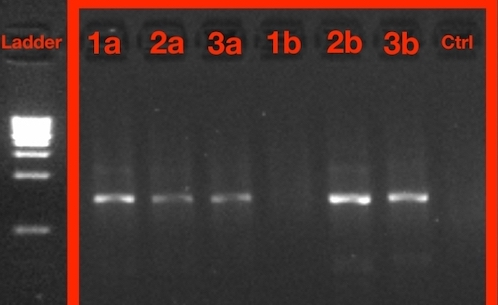
\includegraphics{data/images/gel_images/2019-09-18_Culture_PCRs_BIOL422_Zimmerman_.jpg}
\caption{Gel Electrophoresis for Culture Data taken on September 11,
2019}
\end{figure}

\textbf{Figure 1:} Image of Gel Electrophoresis for Culture Data. PCR
bands corresponding from samples 1A, 2A, 3A, 1B, 2B, 3B, and control
(left to right) are shown within the red box highlighted. A ladder is
shown (furthest to the left) for comparison.

The final gel electrophoresis showcased strong bands are seen in samples
1A, 2B,and 3B. 2A and 3A were described as light bands but are still
prominently shown. However, 1b and the control failed to run at all,
producing no bands.

\hypertarget{image-for-culture-free-data}{%
\subsubsection{Image for Culture Free
Data}\label{image-for-culture-free-data}}

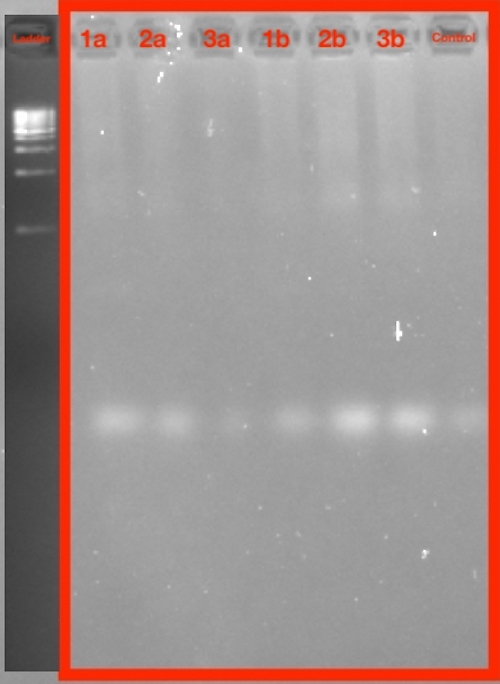
\includegraphics{data/images/gel_images/2019-09-25_Culture_free_PCRs_BIOL422_Zimmerman.jpg}
\textbf{Figure 2:} Image of Gel Electrophoresis for Culture Free Data.
Each PCR bands corresponds to the samples 1A, 2A, 3A, 1B, 2B, 3B, and
control (left to right) are shown within the red box highlighted. A
ladder is also present (furthest to the left) for comparison.

This final gel was different in comparison to the Culture Data (Figure
1) as these bands appeared much lower within the gel. Bands for 1a, 2a,
1b, and the control all appeared very faintly in comparison to 2b and 3b
which were much more distinct white bands. The sample, 3a, appeared most
lightly on the gel in comparison to the other run bands.

These gel images show how the DNA within the samples were separated
based on size and charge. This was also done to help indicate whether
our PCR protocol would work by confirming that the samples had contained
DNA which resulted in this formed bands.

\hypertarget{culture-data}{%
\subsection{Culture Data}\label{culture-data}}

After ensuring that my samples had run to completion, I also wanted to
quantify my culture data for any statistically significant results
between my two sample groups by using my previously collected data for
counting colony abundances. This data was taken after analyzing my Petri
TSA plate samples, using the sample dilutions with the most amount of
data.

From this collected data, I used a box plot to see the average and any
outliers within my data. I also used a statistical test in order to
determine how statistically significant my results were. This would
allow me to make a confident conclusion as to how to interpret my data.

\hypertarget{culture-data-colony-100x-box-plot}{%
\subsubsection{Culture Data Colony 100x Box
Plot}\label{culture-data-colony-100x-box-plot}}

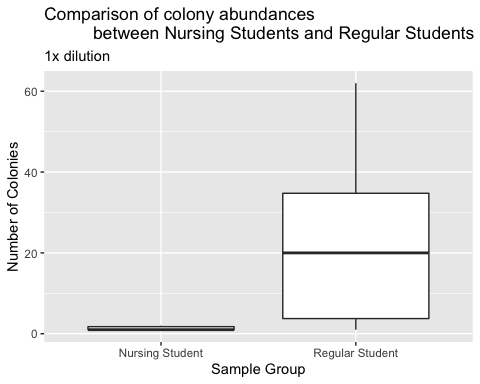
\includegraphics{Bioinformatics_Report_files/figure-latex/filter-and-plot-abundances-1.pdf}

\textbf{Figure 3:} Boxplot of colony abundances at different sites, 1x
dilution. The higher median number, and total number, of colonies from
Regular Students versus Nursing Students was statistically significantly
between the two sites (Wilcox p = 0.03650, rejec the null hypothesis).

\begin{longtable}[]{@{}rrll@{}}
\toprule
statistic & p.value & method & alternative\tabularnewline
\midrule
\endhead
5 & 0.0365039 & Wilcoxon rank sum test with continuity correction &
two.sided\tabularnewline
\bottomrule
\end{longtable}

I also wanted to look at the different types of morphotypes that
appeared from each sample. Using a different variable other than colony
abundances was important as colony morphotypes is a common measurement
for diversity and/or isolation of the dominant species within bacterial
communities (Lebaron \emph{et al.}, 1998). Colony morphotypes can also
be used to identify different species for physiological and genetic
purposes (Lebaron \emph{et al.}, 1998).

\hypertarget{culture-data-morphotype-100x-box-plot}{%
\subsection{Culture Data Morphotype 100x Box
Plot}\label{culture-data-morphotype-100x-box-plot}}

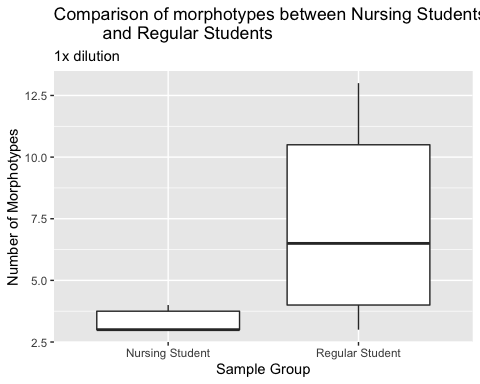
\includegraphics{Bioinformatics_Report_files/figure-latex/filter-and-plot-morphotypes-1.pdf}

\textbf{Figure 4:} Boxplot showing the number of morphotypes from the
two different sites. Nusing students morphotypes averaged
\textgreater{}5, while regulat students had an average of
\textasciitilde{}7 morphotypes. There was a difference in the mean
number of morphotypes (Wilcox p = 0.05, reject the null hypothesis).

\begin{longtable}[]{@{}rrll@{}}
\toprule
statistic & p.value & method & alternative\tabularnewline
\midrule
\endhead
6 & 0.0516086 & Wilcoxon rank sum test with continuity correction &
two.sided\tabularnewline
\bottomrule
\end{longtable}

Boxplots from culture data show that the number of colonies between the
two groups (Group A - Nursing, Group B - Regular) were statistically
different (p = 0.0365, Figure 3). Also seen in the number of
morphotypes, their was also a statistically significant that suggests
evidence of rejecting the null hypothesis due to p = 0.05 (Figure 4).
This data confirms that there the higher number ofcolonies and different
morphotypes within Group B (regular college students) in comparison to
Group A (nursing students) is statistically significant.

\hypertarget{sequencing}{%
\subsection{Sequencing}\label{sequencing}}

As my samples werent sent to a lab and returned as sequenced DNA files,
each DNA file was analyzed as whether they had failed or ran completely.
Files that ran completely were cleaned and trimmed to be adjusted. I
organized my data into a table in order to properly categorize and
document the edits that were made to each successful sequence.

\hypertarget{table-for-each-of-my-sequences}{%
\subsection{Table for each of my
sequences}\label{table-for-each-of-my-sequences}}

\begin{longtable}[]{@{}llllll@{}}
\toprule
\begin{minipage}[b]{0.07\columnwidth}\raggedright
Sample ID\strut
\end{minipage} & \begin{minipage}[b]{0.15\columnwidth}\raggedright
Original File Name\strut
\end{minipage} & \begin{minipage}[b]{0.25\columnwidth}\raggedright
Corrected File name\strut
\end{minipage} & \begin{minipage}[b]{0.07\columnwidth}\raggedright
Usability\strut
\end{minipage} & \begin{minipage}[b]{0.14\columnwidth}\raggedright
Length after Trimming\strut
\end{minipage} & \begin{minipage}[b]{0.16\columnwidth}\raggedright
Manually Adjusted Bases\strut
\end{minipage}\tabularnewline
\midrule
\endhead
\begin{minipage}[t]{0.07\columnwidth}\raggedright
1A\strut
\end{minipage} & \begin{minipage}[t]{0.15\columnwidth}\raggedright
1a\_100x\_AJ\_27f\_A10.ab1\strut
\end{minipage} & \begin{minipage}[t]{0.25\columnwidth}\raggedright
1a\_100x\_AJ\_27f\_A10\_AJ\_Failed.ab1\strut
\end{minipage} & \begin{minipage}[t]{0.07\columnwidth}\raggedright
No\strut
\end{minipage} & \begin{minipage}[t]{0.14\columnwidth}\raggedright
N/A\strut
\end{minipage} & \begin{minipage}[t]{0.16\columnwidth}\raggedright
N/A\strut
\end{minipage}\tabularnewline
\begin{minipage}[t]{0.07\columnwidth}\raggedright
2A\strut
\end{minipage} & \begin{minipage}[t]{0.15\columnwidth}\raggedright
2a\_100x\_AJ\_27f\_B10.ab1\strut
\end{minipage} & \begin{minipage}[t]{0.25\columnwidth}\raggedright
2a\_100x\_AJ\_27f\_B10\_AJ\_Failed\_Blast.ab1\strut
\end{minipage} & \begin{minipage}[t]{0.07\columnwidth}\raggedright
No\strut
\end{minipage} & \begin{minipage}[t]{0.14\columnwidth}\raggedright
N/A\strut
\end{minipage} & \begin{minipage}[t]{0.16\columnwidth}\raggedright
N/A\strut
\end{minipage}\tabularnewline
\begin{minipage}[t]{0.07\columnwidth}\raggedright
3A\strut
\end{minipage} & \begin{minipage}[t]{0.15\columnwidth}\raggedright
3a\_100x\_AJ\_27f\_C10.ab1\strut
\end{minipage} & \begin{minipage}[t]{0.25\columnwidth}\raggedright
2b\_1x\_AJ\_27f\_E10\_AJ Cleaned.ab1\strut
\end{minipage} & \begin{minipage}[t]{0.07\columnwidth}\raggedright
Yes\strut
\end{minipage} & \begin{minipage}[t]{0.14\columnwidth}\raggedright
520\strut
\end{minipage} & \begin{minipage}[t]{0.16\columnwidth}\raggedright
2\strut
\end{minipage}\tabularnewline
\begin{minipage}[t]{0.07\columnwidth}\raggedright
1B\strut
\end{minipage} & \begin{minipage}[t]{0.15\columnwidth}\raggedright
1b\_1x\_AJ\_27f\_D10.ab1\strut
\end{minipage} & \begin{minipage}[t]{0.25\columnwidth}\raggedright
1b\_1x\_AJ\_27f\_D10\_AJ\_Failed.ab1\strut
\end{minipage} & \begin{minipage}[t]{0.07\columnwidth}\raggedright
No\strut
\end{minipage} & \begin{minipage}[t]{0.14\columnwidth}\raggedright
N/A\strut
\end{minipage} & \begin{minipage}[t]{0.16\columnwidth}\raggedright
N/A\strut
\end{minipage}\tabularnewline
\begin{minipage}[t]{0.07\columnwidth}\raggedright
2B\strut
\end{minipage} & \begin{minipage}[t]{0.15\columnwidth}\raggedright
2b\_1x\_AJ\_27f\_E10.ab1\strut
\end{minipage} & \begin{minipage}[t]{0.25\columnwidth}\raggedright
2b\_1x\_AJ\_27f\_E10\_AJ Cleaned.ab1\strut
\end{minipage} & \begin{minipage}[t]{0.07\columnwidth}\raggedright
Yes\strut
\end{minipage} & \begin{minipage}[t]{0.14\columnwidth}\raggedright
518\strut
\end{minipage} & \begin{minipage}[t]{0.16\columnwidth}\raggedright
8\strut
\end{minipage}\tabularnewline
\begin{minipage}[t]{0.07\columnwidth}\raggedright
3B\strut
\end{minipage} & \begin{minipage}[t]{0.15\columnwidth}\raggedright
3b\_1x\_AJ\_27f\_F10.ab1\strut
\end{minipage} & \begin{minipage}[t]{0.25\columnwidth}\raggedright
3b\_1x\_AJ\_27f\_F10\_AJ\_Cleaned.ab1\strut
\end{minipage} & \begin{minipage}[t]{0.07\columnwidth}\raggedright
Yes\strut
\end{minipage} & \begin{minipage}[t]{0.14\columnwidth}\raggedright
496\strut
\end{minipage} & \begin{minipage}[t]{0.16\columnwidth}\raggedright
2\strut
\end{minipage}\tabularnewline
\bottomrule
\end{longtable}

\textbf{Table 2:} Table showing the locus of each sequence (16S),
original filename of each sequence, the filename after correcting or
marking as failed, its usability (useable vs unusable), length after
trimming, and number of manually corrected in the remaining sequence
after trimming.

Successful sequences were 3A, 2B, and 3B. The other sequences had failed
to run code (showing 'NNNN only) or had too much noise (2A). The data
was then trimmed and sequenced to be ready for alignment with the
outgroup \emph{Thermus aquaticus} strain YT-1 16 S. Any ambiguity was
manually corrected following
\href{https://droog.gs.washington.edu/parc/images/iupac.html}{the IUPAC
ambiguity code}.

\hypertarget{table-for-each-of-my-successful-sanger-sequences-after-blast}{%
\subsection{Table for each of my successful Sanger Sequences after
BLAST}\label{table-for-each-of-my-successful-sanger-sequences-after-blast}}

\begin{longtable}[]{@{}llllll@{}}
\toprule
Sample & Description & Percent Identity & Query Cover & Ascension & E
Value\tabularnewline
\midrule
\endhead
1A & Sequence Failed & & & &\tabularnewline
2A & Sequence Failed & & & &\tabularnewline
3A & Moraxella Osloensis Strain PK2-16.2 & 98.65\% & 99\% & MN428170.1 &
0.0\tabularnewline
1B & Sequence Failed & & & &\tabularnewline
2B & Straphylococcus warneri strain SR5-28 & 99.61\% & 100\% &
MN421516.1 & 0.0\tabularnewline
3B & Acinetobacter sp. strain GR14 16S & 100\% & 100\% & MH883927.1 &
1e-139\tabularnewline
\bottomrule
\end{longtable}

\textbf{Table 3:} Table of successful Sanger Sequences after NCBI BLAST
Results. This table indiccates the BLAST result metricts which include
description, percent identiy, query cover, ascension and E value.

All results from the Table were taken from NCBI Gene Bank. Each
successful sequence had a high percent identity with its match found. 3A
was matched with the \emph{Moraxella osloensis} strain, 2B with the
\emph{Straphylococcus warneri} strain, and finally 3B had the
\emph{Acinetobacter} strain. Other strains had failed to sequence
therefore not coming with any matches.

\hypertarget{phylogenies}{%
\subsection{Phylogenies}\label{phylogenies}}

Following successful sequencing, my sequences were then aligned for
proper phylogenetic analysis using Geneious Prime. My phylogenetic trees
represent the relatedness between my sequences and the outgroup,
\emph{Thermus aquaticus}. Phylogenies allow for easier identification of
the bacteria found on my samples. Two phylogenetic trees were created
using different methods of construction, PhyML and Mr.~Bayes.

\hypertarget{phyml-phylogenetic-tree}{%
\subsubsection{PhyML Phylogenetic Tree}\label{phyml-phylogenetic-tree}}

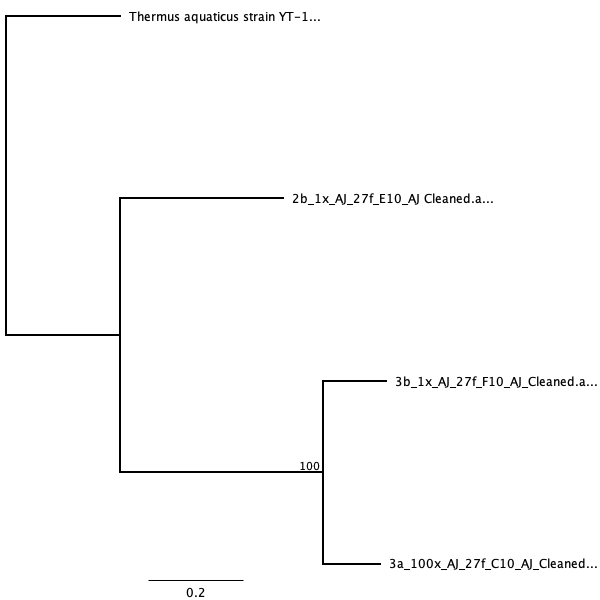
\includegraphics{output/phylogenies/Sanger_Sequence_PHYML_Phylogeny.png}
\textbf{Figure 5:} PhyML Phylogenetic tree run on Geneious Prime from
Sanger Sequencing Data. Sequences that ran are 3A, 2B, and 3B with an
outgroup of \emph{Thermus aquaticus} Strain YT-1 16 S.

\hypertarget{mr.bayes-phylogenetic-tree}{%
\subsubsection{Mr.~Bayes Phylogenetic
tree}\label{mr.bayes-phylogenetic-tree}}

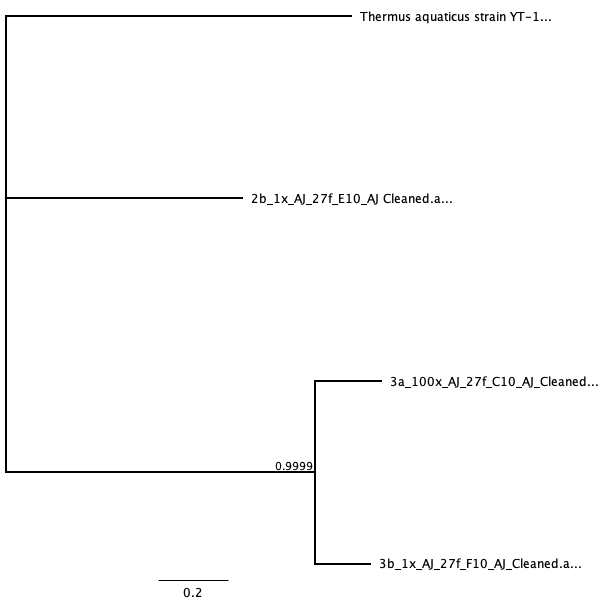
\includegraphics{output/phylogenies/Sanger_Sequence_MrBayes_Phylogeny.png}
\textbf{Figure 6:} Mr.~Bayes Phylogenetic tree run on Geneious Primer
from Sanger Sequencing Data. Sequences that ran are 3A, 2B, and 3B with
an outgroup of \emph{Thermus aquaticus} Strain YT-1 16 S.

The PhyML Tree used the parammeters of substitution model of GTR with a
value of 100 Bootstraps. Mr.~Bayes ran also under GTR, a rate variation
of invgamma, a chain length of 1,100,000, a subsampling freq of 200, and
a burn-in length of 100,000. Phylogenetic differences between the two
trees are based on the placement of 2b in relation to the related 3A and
3B and the outgroup. I found that both trees strongly associate 3A and
3B together with PhyML tree's bootstrap value of 100 and Mr.~Bayes is
about 0.999 (Figure 5, 5, ML bootstrap 100 \textasciitilde{}= Bayes
0.999). While PhyML associates 2B more closely related to 3A and 3B,
Mr.~Bayes places 2B alongside the outgroup.

\hypertarget{fastqc-report}{%
\subsection{FastQC Report}\label{fastqc-report}}

\begin{longtable}[]{@{}cccc@{}}
\toprule
File Name & Sequences Flagged as Poor Quality & Sequence Length &
\%GC\tabularnewline
\midrule
\endhead
AJ-1a\_S61\_L001\_R1\_001 & 0 & 147-151 & 52\%\tabularnewline
AJ-1b\_S64\_L001\_R1\_001 & 0 & 147-151 & 52\%\tabularnewline
AJ-2a\_S62\_L001\_R1\_001 & 0 & 41-151 & 53\%\tabularnewline
AJ-2b\_S65\_L001\_R1\_001 & 0 & 146-151 & 52\%\tabularnewline
AJ-3a\_S63\_L001\_R1\_001 & 0 & 42-151 & 53\%\tabularnewline
AJ-3b\_S66\_L001\_R1\_001 & 0 & 41-151 & 53\%\tabularnewline
\bottomrule
\end{longtable}

\textbf{Table 4:} Table of the data taken from FastQC reports. Data
showcased any sequences flagged as poor quality (failure to run),
sequence length, and \%GC (Count(G + C)/Count(A + T + G + C) * 100\%.).
1A (Nursing Student) had a sample file name of
AJ-1a\_S61\_L001\_R1\_001, 1B: AJ-1b\_S64\_L001\_R1\_001 (Regular
Student), 2A (Nursing Student): AJ-2a\_S62\_L001\_R1\_001, 2B:
AJ-2b\_S65\_L001\_R1\_001 (Regular Student), 3A (Nursing Student):
AJ-3a\_S63\_L001\_R1\_001, and 3B: AJ-3b\_S66\_L001\_R1\_001 (Regular
Student).

When looking at FastQC Reports, it is important to look at the Quality
Control of the file, also known as the level of quality of the Illumina
Sequences ran. Each of my sequences were not flagged for poor quality
and was regarded as a successful run. I lalso ooked at Sequence Length
as an indicator of the length of the shortest and longest sequence
within the set. AJ-1a\_S61\_L001\_R1\_001 and AJ-1b\_S64\_L001\_R1\_001
both had the same Sequence Length of 147-151 while
AJ-2a\_S62\_L001\_R1\_001 and AJ-3b\_S66\_L001\_R1\_001 also had the
same length of 41-151. AJ-2b\_S65\_L001\_R1\_001 and
AJ-3a\_S63\_L001\_R1\_001 had sequence lengths that were one off from
the first two groups respectively. I also looked at \%GC which indicates
the overall \%GC of all bases in all sequences. This is reported as all
counted G and C base pairs over total count of all possible base pairs
(Count(G + C)/Count(A + T + G + C) * 100\%.).Sequences
AJ-1a\_S61\_L001\_R1\_001, AJ-1b\_S64\_L001\_R1\_001, and
AJ-2b\_S65\_L001\_R1\_001 had a \%GC of 52\% while the rest of the
sequences had 53\%. All \%GC were within the range to have all the
sequences be regarded as quality sequences.

\hypertarget{trimmmomatic-data}{%
\subsection{Trimmmomatic Data}\label{trimmmomatic-data}}

\begin{longtable}[]{@{}cccc@{}}
\toprule
Sample ID & Before Trimming & After Trimming & Percentage
Survived\tabularnewline
\midrule
\endhead
AJ-1a\_S61\_L001\_R1\_001 & 8428 & 7891 & 93.62\%\tabularnewline
AJ-1b\_S64\_L001\_R1\_001 & 11693 & 11129 & 95.18\%\tabularnewline
AJ-2a\_S62\_L001\_R1\_001 & 7788 & 7310 & 93.86\%\tabularnewline
AJ-2b\_S65\_L001\_R1\_001 & 15715 & 14989 & 95.38\%\tabularnewline
AJ-3a\_S63\_L001\_R1\_001 & 14939 & 14245 & 95.35\%\tabularnewline
AJ-3b\_S66\_L001\_R1\_001 & 13216 & 12393 & 93.77\%\tabularnewline
\bottomrule
\end{longtable}

\textbf{Table 5:} Table showcasing sequence number of each sample ran
(percentage survived = after trimming /before trimming).

Trimmomatic was done from a for loop on the terminal line to trim down
the sample sequences. `Before Trimming' data was taken from the FastQC
reports under `Total Sequences' for each sample. Total sequences is a
count of the total number of sequences processed. `After Trimming' data
was taken from the command line using the grep-c function within my
illumina sequence data. Percentage survived average these two data sets.
Samples AJ-1b\_S64\_L001\_R1\_001, AJ-2b\_S65\_L001\_R1\_001,
AJ-3a\_S63\_L001\_R1\_001 were able to keep around 95\% of the original
sequences. While samples AJ-1a\_S61\_L001\_R1\_001,
AJ-2a\_S62\_L001\_R1\_001, and AJ-3b\_S66\_L001\_R1\_001 kept around
93\% of their original sequence. All samples maintained a high
percentage survival which indicated that all sequences successfully ran.

\hypertarget{command-line-blast-analysis}{%
\subsection{Command-line BLAST
Analysis}\label{command-line-blast-analysis}}

\begin{figure}
\centering
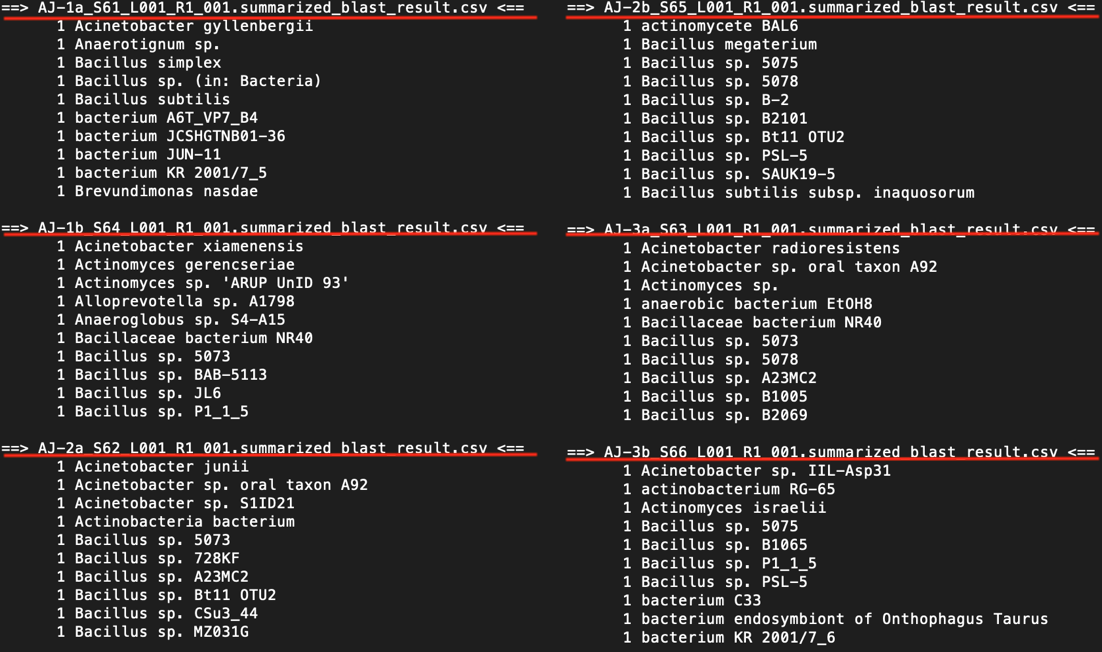
\includegraphics{data/images/Illumina_BLAST_result/Illumina-Sequences-BLAST-Summary.png}
\caption{Final BLAST result for Illumina Sequences}
\end{figure}

\textbf{Figure 7:} Image showcasing final BLAST result from fasta
Illumina sequence sample files on the command-line Terminal. All
sequences are highlighted in red or indicated via the arrow. Each
sequence had BLASTed for 10 different bacteria types with 1 of each
bacteria listed below each line (n=6 sequences, 60 different bacteria
listed ).

All Illumina Sequences for the samples successfully ran and were able to
be processed for BLAST sequencing. The result of this BLAST showed 10
different bacteria types for each of my Illumina sequences. As each of
the samples equally had same amount of sequences for each taxa of
bacteria for each set of 10, trends were analyzed between each sample.
All sequences except for AJ-2b\_S65\_L001\_R1\_001 had tested for a type
of \emph{Acinetobacter}. While all of the samples had a BLAST result of
a certain type of \emph{Bacillus} or \emph{Bacillaceae} were present in
their sequences. The genus \emph{Bacterium} was only present in
AJ-1a\_S61\_L001\_R1\_001 and AJ-3b\_S66\_L001\_R1\_001.
\emph{Actinomyces} or \emph{actinmyocete} were present in
AJ-1b\_S64\_L001\_R1\_001, AJ-2b\_S65\_L001\_R1\_001,
AJ-3a\_S63\_L001\_R1\_001. AJ-1a\_S61\_L001\_R1\_001 had the unique
bacteria of \emph{Alloprevotella sp A1798} and \emph{Brevundimos
nasdae}. Other sequences with unique bacteria were
AJ-1b\_S64\_L001\_R1\_001 with \emph{Alloprevotella sp. A1789} and
\emph{Anaeroglobus sp. 54-A15} and AJ-3a\_S63\_L001\_R1\_001 with
\emph{Anaerobic bacterium EtOH8}. \# Discussion

\hypertarget{summary}{%
\subsection{Summary}\label{summary}}

Mobile phones have become one of the indispensable accessories in
everyday modern life (Karabay \emph{et al.}, 2007). Cell phones are
taken with us everywhere even in hospital halls, laboratories, and/or
intensive care units when dealing with severe illnesses (Karabay
\emph{et al.}, 2007). Moreover, college students were also noted to not
only take their phones everywhere, but also are exposed to the most
among germs do the density of college campuses and students (Ross and
Neufeld, 2015). Thus, my study attempted to analyze whether college
students who do enter hospitals (such as Nursing students) have the
potential at being bacterial carriers for infections due to their cell
phone use. Specifically, I had sampled the phones of 6 total college
students at the University of San Francisco, 3 of which were Nursing
students working at the clinical site at Saint Mary's Hospital while the
other 3 were just regular non-health related students. I had wanted to
see whether Nursing students did sanitize their phones and take extra
precautions in limiting their bacterial contact in comparison to regular
college students. I hypothesized that Nursing students were required to
clean their phones, thus showing less bacterial growth.

My Culture data confirmed my hypothesis statistically as there was a
reported difference in the number of colonies found between the two
groups (Figure 3), and in the number of morphotypes with the colonies
(Figure 4). However, insterestingly I found that the bacteria found in
the phones of the regular students (2B and 3B) indicated bacteria that
were just as likely to be infectious than the bacteria found from the
nursing student (3A). 2B showed up as the \emph{Staphylococcus warneri}
strain and 3B was the \emph{Acinetobacter sp. strain}, while 3A had
matched as the \emph{Moraxella osloensis} strain. This contradicted
previous studies which indicated that those who worked in the medical/
healthcare setting had much more resistant and dangerous bacteria found
within their phones (Taher, 2019). While there was no complete
indication that Nursing students had fewer bacteria than regular
students, it was evident that Nursing students (Group A) had much fewer
morphotypes in the colonies found in Group B. This data provided some
evidence that Nursing students, at least the University of San
Francisco, have much better safety precaution against high levels of
bacterial growth in comparison to regular college students.

My Culture Free data also confirmed the idea that each of the species
identified on cell phones were just as likely to be as infectious as the
other regardless of whether the cell phone belonged to a Nursing Student
or Regular Student. All sequences (except for the sequence of sample 2B:
AJ-2b\_S65\_L001\_R1\_001) had tested for a type of \emph{Acinetobacter}
and all of the samples had a type of \emph{Bacillus} or
\emph{Bacillaceae}. These species are common for types of bacterium and
can be a harmful pathogen for infectious diseases depending on the
specific taxa. One interesting result from almost all samples testing
for \emph{Acinetobacter}, is that \emph{Acinetobacter} are gram-negative
organisms that can cause infections in any organ system often found
within hospitalized patients and the fact that it was also present in
all of the Regular Students indicated that the level of how harmful/
infectious the pathogen present on a cell phone did not differ on
whether the cell phone user was exposed to the hospital setting as a
Nursing student or a Regular student . The species of \emph{Bacillus}
also has a clinical spectrum of infections which include things like
food poisoning, localized infections related to trauma, deep seated soft
tissue infections, and systemic infections (Weber \emph{et al.}, 1988).
Thus, a majority of my Culture Free data contradicted my original idea
that Regular Students would have more harmful bacteria due to their lack
of sanitization, but instead shows that regardless of group type (A:
Nursing students, B: Regular students) all samples tested for similar
bacterial types.

The end result of my report showed that while Regular Students had
statistically shown a significant amount of bacterial colonies and
morphotypes compared to Nursing Students, the level of how harmful/
infectious the bacteria (or bacteria type) did not differ between the
two groups. While Nursing Students had less bacteria due to their
sanitizing protocols, there is still the potential for the student to
bring in an HAI into a hospital setting. Thus, further study on
different sanitizing methods to properly kill off a majority of these
infectious strains is required to come up with a better way of
protecting hospital patients and workers.

\hypertarget{interpretation-of-sanger-sequencing-and-taxa}{%
\subsection{Interpretation of Sanger Sequencing and
Taxa}\label{interpretation-of-sanger-sequencing-and-taxa}}

From my evidence found in Figure 4, it can be interpreted that there are
many more types of bacteria and amount of colonies growing on regular
students' cell phones in comparison to the Nursing students. This could
be due to the fact that Nursing students are found in the sterile
environment, and as pointed from the data that they do clean their
phones, they are more likely to come across the same type of bacteria
rather than regular college students who can go around anywhere without
worrying about sanitizing. There is also the interpretation that the
number of colonies may not be as indicative when comparing the
``cleaner'' phone (fewer bacteria), as colony growth can vary between
types of bacteria whether it be based on environment, growth rate,
conditions, temperature. Thus, I found the number of morphotypes to be
more indicative of the difference between nursing students and regular
students.

However, the difference between the two groups could easily be
manipulated based on uncontrollable variances in each student's life.
For example, one student could use their phones much more carelessly by
placing it on dirty surfaces, letting it stay on the floor, while
another student could keep their phones in their backpacks for the day.
There could also be differences in lifestyles as nursing students, like
someone being on their phone during clinical site, while the other keeps
it in their pocket most of the time. There was also a difference in
livelihood like someone living in the dorms or a crowded house, visiting
the gym more often, or even general body hygiene (such as washing
hands). While I do think my data is statistically significant, it is
also important to consider all possibilities when considering the two
groups.

It was also interesting to see the data from Table 3 that indicates the
BLAST matches of each successfully ran sequence (3A, 2B, 3B). From these
sequences and the bacteria associated, it is also easier to interpret
the phylogenetic trees (Figures 4, 5). I agreed that both trees had
correctly placed 3A and 3B together due to the high bootstrap values of
PhyML tree's being 100 and Mr.~Bayes is about 0.999 (Figure 5, 5, ML
bootstrap 100 \textasciitilde{}= Bayes 0.999). While PhyML associates 2B
more closely related to 3A and 3B, Mr.~Bayes places 2B alongside the
outgroup. This can be better interpreted through understanding the
epidemiology of exactly the bacteria that most matched my data from the
NCBI genebank BLAST tool was. I found that the \emph{Staphylococcus
warneri} strain most matched my sample 2B, 3B as the Acinetobacter sp.
strain, and 3A was most matched to the \emph{Moraxella osloensis}
strain. As previously mentioned, each bacteria was found to be just as
probable for infection if spread and contaminated.

While I agree with the bootstrap values of my phylogenetic tree, it was
hard to actually pinpoint what made 3A and 3B much more closely related
in comparison to 2B. I did mention that each of the bacteria strands was
just as probable for infection, there were differences in the severity
of each infection. For sample 2B, \emph{Staphylococcus warneri}, it is a
member of the bacterial genus \emph{Staphylococcus} which can cause
infection in patients whose immune system is compromised (Campoccia
\emph{et al.}, 2010). \emph{S. warneri} causes infectious usually in
association due to implant materials, orthopedic infections, or the
absence of a foreign body (2010) orthopedic infections. Also dealing
with skin and epithelium, the \emph{Moraxella osloensis}, found as 3A,
is also a gram-negative bacterium that is saprophytic on skin and mucosa
(Lim \emph{et al.}, 2018). This strain, like the \emph{Staphylococcus},
is frequently involved in human infectious diseases (2018). Found in 3B,
**Acinetobacter* is also the genus of Gram-negative bacteria belonging
to the wider class of \emph{Gammaproteobacteria} which are known to
cause high mortality infections like its strand \emph{A. baumannii} with
high virulence and antimicrobial resistance (Kuo). \emph{Acinetobacter
spp.} first began to be recognized as significant healthcare-associated
pathogens during the 1970s and many of these infections involve
multidrug-resistant strains and occur in intensive care or
high-dependency units in which severely-ill or debilitated patients are
treated extensively with broad-spectrum antibiotics . Thus, based on
where the bacteria attacks, it would be more considerable that 2B and 3A
were more closely related than 3A and 3B based on the level of
virulence. However, after more research, \emph{Staphylococcus} was less
likely to be as deadly as 3A and 3B when it comes to being infectious.
Thus, from my data, it can be interpreted that 3A and 3B are more
closely related as seen in Figures 4 and 5, while 2B is more closely
related to the outgroup the \emph{Thermus aquaticus.} To determine how
much closer related 2B was to the outgroup, a study done by Delarue et.
al stuck out in which they looked at the polymerase sequence from
bacteriophage and found that to be homologous to the polymerase domain
of polymerase I from Escherichia coli, which is also closely related to
those from \emph{Staphylococcus pneumoniae}, \emph{Thermus aquaticus}
(Delarue \emph{et al.}, 1990). Thus, the shared homology with this
bacteriophage that Delarue et. al looked at also indicates a link
between Staphyloccocus and \emph{Thermus aquaticus}. From this study,
the correct taxa from my data are seen within my Mr.~Bayes phylogenetic
tree (Figure 6).

\hypertarget{interpretation-of-illumina-sequencing-and-taxa}{%
\subsection{Interpretation of Illumina Sequencing and
Taxa}\label{interpretation-of-illumina-sequencing-and-taxa}}

Each of my Culture Free samples were able to properly sequence and run
through BLAST with high quality reads (Table 4, 5). Each of the samples
also listed for 10 different bacterium with equivalent presence in each
sample (Figure 7).

In contrast with my Culture data, 2B did not show up as the
\emph{Staphyloccus warneri} strand, but instead had a BLASTed for
\emph{actinmyocete BAL6} and other types of \emph{Bacillus} bacterium
(Figure 7). 3B did test for an \emph{Acinetobacter sp. strain}, but this
result singled out \emph{Acinetobacter sp. IIL-Asp31}. 3A did not
sequence for any \emph{Moraxella osloensis} strain, but instead tested
for \emph{Acinetobacter}, \emph{Actinmyces}, \emph{Anaerobic Bacterium
EtOH8}, and other \emph{Bacillus} (Figure 7). The main difference
between the newly BLASTed bacterium from my Illumina Sequences in
comparison to my BLASTed Sanger Sequences is that 2B, 3B, and 3A all
also had similar genera for their identified bacterium (either
\emph{Acinetobacter} and \emph{Bacillus}). This contradicts previous
studies that Nursing Students had less infectious pathogens within their
cell phones, as the common genera amongst all samples were all
potentially infectious.

I am much more confident in these newly resulting identified bacterium
due to the fact that the Culture Free data relied on Illumina Sequencing
rather than Sanger Sequencing. This is important because Sanger
sequencing only allows for a single DNA fragment at a time, while
Illumina Sequencing, a type of Next Generation Sequencing, can sequence
millions of fragments simultaneously per run. Illumina Sequencing is
considered a high-throughput process which results in a more with deep
sequencing, which gives me much more confidence in the bacteria
identified from my Culture Free data rather than my Cultured.

What was most interesting from Figure 7 was that all sequences for the
Regular Students (1B, 2B, 3B) had tested for a type of
\emph{Actinomyces} or \emph{actinomycete}. This was important as
actinomycosis is a rare chronic disease caused by the
\emph{Actinomyces}, an anaerobic Gram-positive bacteria that normally
colonize the human mouth and digestive and genital tracts (Kim \emph{et
al.}, 2014). While 3A also tested for \emph{Actinomyces sp.}, the
majority trend of Regular Students all containing the pathogen provided
potential evidence that could have supported my hypothesis that Regular
Students would have a greater number of harmful pathogens. However, from
the other similar types of genera present in all samples, I came to the
conclusion that all types of bacterium can occur on any type of phone,
regardless of profession or the frequency of cell phone sanitization.

\hypertarget{error-analysis}{%
\subsection{Error Analysis}\label{error-analysis}}

Due to the low number of actual sequencing DNA, it can be interpreted
that there may have been something wrong during collection, extraction,
PCR protocol, or even sequencing and everything in between (Table 2).

Key data points that may have resulted in a lack of successful
sequencing could be due to experimental error. During PCR Protocol, my
master mix had actually run out before the 19 ul could be delivered to
each sample. Instead, I had decided to modify the procedure and use 17
ul. Thus, there could be an indication that there was not enough
template for the sequence to amplify. My data also showed a lot of
compression among sequences indicating DNA fragments of different sizes
with the same electrophoretic mobility, ie fragments that migrate on top
of each other during electrophoresis (Dillon). This phenomenon is
thought to be caused by regions of secondary structure within the
template DNA which could be due to PCR not having high enough
temperature for denaturing. Also notable, my gel electrophoresis already
indicated a failure in 1B (Figure 1), which coincides with the idea that
my sequences failed to run. There were also issues with editing my
sequences as a lot of them were judgment calls. This could have caused
change base pairs that were manipulated to better fit one bacteria more
as opposed to another. This could also have skewed the placement of my
phylogenetic tree.

Other evidence of experimental failure could be due to
cross-contamination, whether it be from extracting too much TSA when
scraping the culture from the culture plates or by not being extra
cautious when using pipette tips and handling other tools. As my Qubit
data showed high numbers in the correct range, there is also the
possibility that the bacteria that are found on the phones are resistant
to PCR, air, water-- indicating that there is a lot of versatility in
bacteria that my protocol could not account for. If that is the case,
PCR could be redone at high temperatures to ensure complete denaturing
of the DNA strands and longer cycles for higher amplification.

Any other error in data from my Culture Free samples would be due to
machine error. This can be attributed to any errors within command line
(such as improper git pushes and cloning) or simple program errors from
R Markdown or any other terminal commands. Other issues can be due to
poor server connection when attempting to access the Tule sever within
the University of San Francisco Network.

\hypertarget{sources-cited}{%
\section*{Sources Cited}\label{sources-cited}}
\addcontentsline{toc}{section}{Sources Cited}

\hypertarget{refs}{}
\leavevmode\hypertarget{ref-amplicon201316s}{}%
Amplicon,P. \emph{et al.} (2013) 16s metagenomic sequencing library
preparation.

\leavevmode\hypertarget{ref-bolger2014trimmomatic}{}%
Bolger,A.M. \emph{et al.} (2014) Trimmomatic: A flexible trimmer for
illumina sequence data. \emph{Bioinformatics}, \textbf{30}, 2114--2120.

\leavevmode\hypertarget{ref-campoccia2010characterization}{}%
Campoccia,D. \emph{et al.} (2010) Characterization of 26 staphylococcus
warneri isolates from orthopedic infections. \emph{The International
journal of artificial organs}, \textbf{33}, 575--581.

\leavevmode\hypertarget{ref-delarue1990attempt}{}%
Delarue,M. \emph{et al.} (1990) An attempt to unify the structure of
polymerases. \emph{Protein Engineering, Design and Selection},
\textbf{3}, 461--467.

\leavevmode\hypertarget{ref-dillon}{}%
Dillon,C. Troubleshooting dna sequencing: Evaluating sanger dna
sequencing chromatogram data. \emph{Amplicon Express}.

\leavevmode\hypertarget{ref-guindon2010new}{}%
Guindon,S. \emph{et al.} (2010) New algorithms and methods to estimate
maximum-likelihood phylogenies: Assessing the performance of phyml 3.0.
\emph{Systematic biology}, \textbf{59}, 307--321.

\leavevmode\hypertarget{ref-karabay2007role}{}%
Karabay,O. \emph{et al.} (2007) The role of mobile phones in the spread
of bacteria associated with nosocomial infections. \emph{J Infect Dev
Ctries}, \textbf{1}, 72--3.

\leavevmode\hypertarget{ref-katoh2013mafft}{}%
Katoh,K. and Standley,D.M. (2013) MAFFT multiple sequence alignment
software version 7: Improvements in performance and usability.
\emph{Molecular biology and evolution}, \textbf{30}, 772--780.

\leavevmode\hypertarget{ref-kim2014actinomyces}{}%
Kim,Y.J. \emph{et al.} (2014) Actinomyces-like organisms in cervical
smears: The association with intrauterine device and pelvic inflammatory
diseases. \emph{Obstetrics \& gynecology science}, \textbf{57},
393--396.

\leavevmode\hypertarget{ref-koljalg2017high}{}%
Kõljalg,S. \emph{et al.} (2017) High level bacterial contamination of
secondary school students' mobile phones. \emph{Germs}, \textbf{7}, 73.

\leavevmode\hypertarget{ref-kuo}{}%
Kuo,S.-C. Acinetobacter species. \emph{Acinetobacter species -
Infectious Disease and Antimicrobial Agents}.

\leavevmode\hypertarget{ref-10.1111ux2fj.1574-6968.1998.tb12903.x}{}%
Lebaron,P. \emph{et al.} (1998) Phenotypic and genetic diversity within
a colony morphotype. \emph{FEMS Microbiology Letters}, \textbf{160},
137--143.

\leavevmode\hypertarget{ref-lim2018complete}{}%
Lim,J.Y. \emph{et al.} (2018) Complete genome sequences of three
moraxella osloensis strains isolated from human skin. \emph{Genome
announcements}, \textbf{6}.

\leavevmode\hypertarget{ref-meadow2014mobile}{}%
Meadow,J.F. \emph{et al.} (2014) Mobile phones carry the personal
microbiome of their owners. \emph{PeerJ}, \textbf{2}, e447.

\leavevmode\hypertarget{ref-nwankwo2014nosocomial}{}%
Nwankwo,E. \emph{et al.} (2014) Nosocomial pathogens associated with the
mobile phones of healthcare workers in a hospital in anyigba, kogi
state, nigeria. \emph{Journal of epidemiology and global health},
\textbf{4}, 135--140.

\leavevmode\hypertarget{ref-ross2015microbial}{}%
Ross,A.A. and Neufeld,J.D. (2015) Microbial biogeography of a university
campus. \emph{Microbiome}, \textbf{3}, 66.

\leavevmode\hypertarget{ref-sadat2010bacterial}{}%
Sadat-Ali,M. \emph{et al.} (2010) Bacterial flora on cell phones of
health care providers in a teaching institution. \emph{American journal
of infection control}, \textbf{38}, 404--405.

\leavevmode\hypertarget{ref-sepehri2009bacterial}{}%
Sepehri,G. \emph{et al.} (2009) Bacterial contamination and resistance
to commonly used antimicrobials of healthcare workers' mobile phones in
teaching hospitals, kerman, iran. \emph{American Journal of Applied
Sciences}, \textbf{6}, 806.

\leavevmode\hypertarget{ref-suchard2006bali}{}%
Suchard,M.A. and Redelings,B.D. (2006) BAli-phy: Simultaneous bayesian
inference of alignment and phylogeny. \emph{Bioinformatics},
\textbf{22}, 2047--2048.

\leavevmode\hypertarget{ref-taher2019pathogenic}{}%
Taher,N.M. (2019) Pathogenic bacteria isolated from personal cell phones
of health care staff in iraqi hospitals. \emph{J Pure Appl Microbiol},
\textbf{13}, 1145--1150.

\leavevmode\hypertarget{ref-tajeddin2016role}{}%
Tajeddin,E. \emph{et al.} (2016) The role of the intensive care unit
environment and health-care workers in the transmission of bacteria
associated with hospital acquired infections. \emph{Journal of infection
and public health}, \textbf{9}, 13--23.

\leavevmode\hypertarget{ref-ulger2009we}{}%
Ulger,F. \emph{et al.} (2009) Are we aware how contaminated our mobile
phones with nosocomial pathogens? \emph{Annals of clinical microbiology
and antimicrobials}, \textbf{8}, 7.

\leavevmode\hypertarget{ref-weber1988vitro}{}%
Weber,D.J. \emph{et al.} (1988) In vitro susceptibility of bacillus spp.
To selected antimicrobial agents. \emph{Antimicrobial agents and
chemotherapy}, \textbf{32}, 642--645.


\end{document}
